% Beamer Presentation and Lecture Note Template
% Version 0.1
% by Paul Vesey

\mode<presentation> {
\usetheme{Antibes}
\setbeamercovered{invisible}
\setbeamertemplate{footline}[frame number]
\setbeamertemplate{navigation symbols}{} 
}

\usepackage{eurosym}
\usepackage{graphicx}
\usepackage{wasysym}
\usepackage{hyperref}
\usepackage{amsmath}
\usepackage{amssymb}
\usepackage{mathtools}
\usepackage{tikz}
\usepackage{pgf}
\usepackage{pgfplots}
\usepackage{pxfonts}
\usepackage{textcomp}
\usepackage{verbatim}
\usepackage{color}
\usepackage{xcolor}
\usepackage{fix-cm}


\author{Paul Vesey}
\institute[TUS]
{
Technological University of the Shannon \\
\medskip
{\emph{paul.vesey@tus.ie}}
}
\date{Autumn 2022}



%\usepackage{bm} 
% For typesetting bold math (not \mathbold)
%\logo{\includegraphics[height=0.6cm]{yourlogo.eps}}
%
\title[Project Management \& BIM]{Measurement Performance Domain}


\begin{document}
%
\usetikzlibrary{arrows}
\usepgflibrary{patterns}



\thispagestyle{empty} % Remove page numbering on this page

%----------------------------------------------------------------------------------------
%	TITLE SECTION
%----------------------------------------------------------------------------------------

\hrule

\vspace*{0.7cm} % Space between the start of the title and the top of the grey box


\begin{flushright}
\Huge Project Management \& Building Information Modelling \\
\vspace*{0.7cm}
\Large BSc (Hons) in Construction Management\\
BSc (Hons) in Civil Engineering Management\\
Year 4 (2021-2022)
\end{flushright}

\vspace*{0.7cm} % Space between the end of the title and the bottom of the grey box
	
\normalsize

\hrule

%----------------------------------------------------------------------------------------

\vfill % Space between the title box and author information

%----------------------------------------------------------------------------------------
%	AUTHOR NAME AND INFORMATION SECTION
%----------------------------------------------------------------------------------------

{\centering \large 
\hfill Paul Vesey, \scriptsize BEng (Hons), MIE, HDip\normalsize \\
\hfill Limerick Institute of Technology \\
\hfill Department of the Built Environment \\
\hfill \texttt{https://paulvesey.wordpress.com} \\
\vspace*{0.7cm} 
\hrule} % Horizontal line, thickness changed here

%----------------------------------------------------------------------------------------

\clearpage % Whitespace to the end of the page

\newpage




\thispagestyle{empty}
\tableofcontents
\newpage
\section{Measurement Performance Domain}


\begin{frame}
\titlepage
\end{frame}\begin{center}\line(1,0){250}\end{center}
%
%
\begin{center}\line(1,0){250}\end{center}


\section{Guide}



\begin{frame}
\frametitle{Project ????}
 \begin{figure}
    \centering
        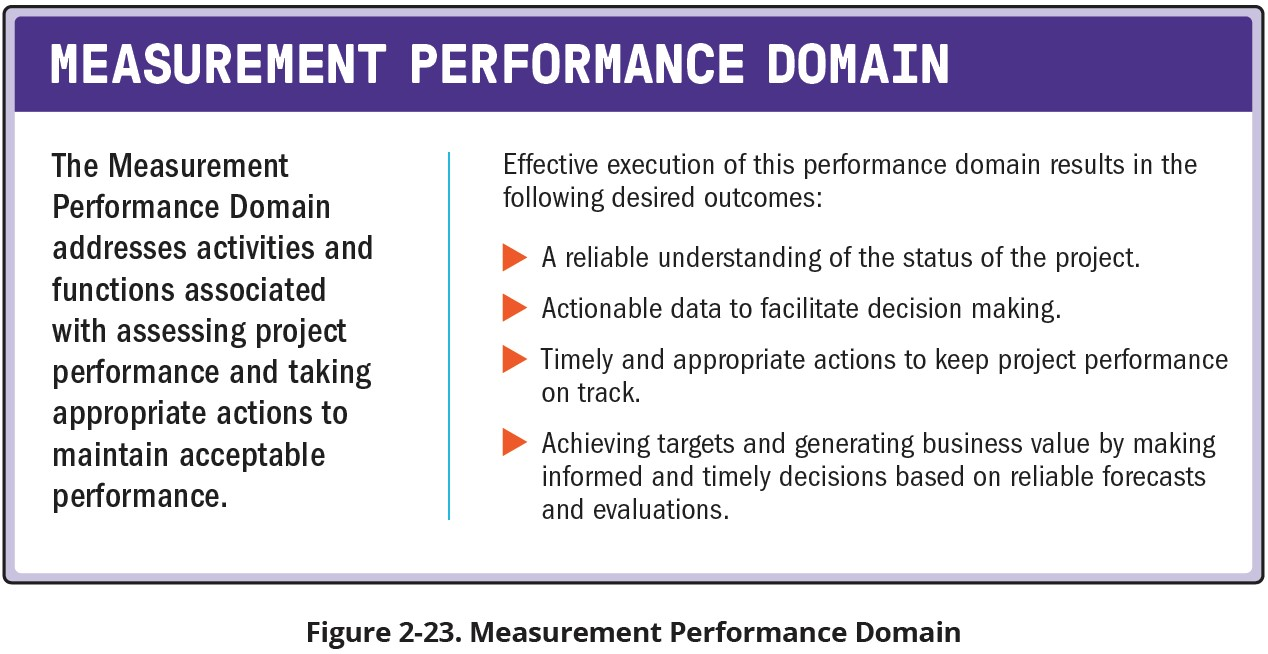
\includegraphics[width = 8cm]{../images/guide/Fig2-23.jpg}
    \label{guidefig:2-23}
 \end{figure}
\end{frame}
\begin{center}\line(1,0){250}\end{center}

\begin{frame}
\frametitle{Project ????}
 \begin{figure}
    \centering
        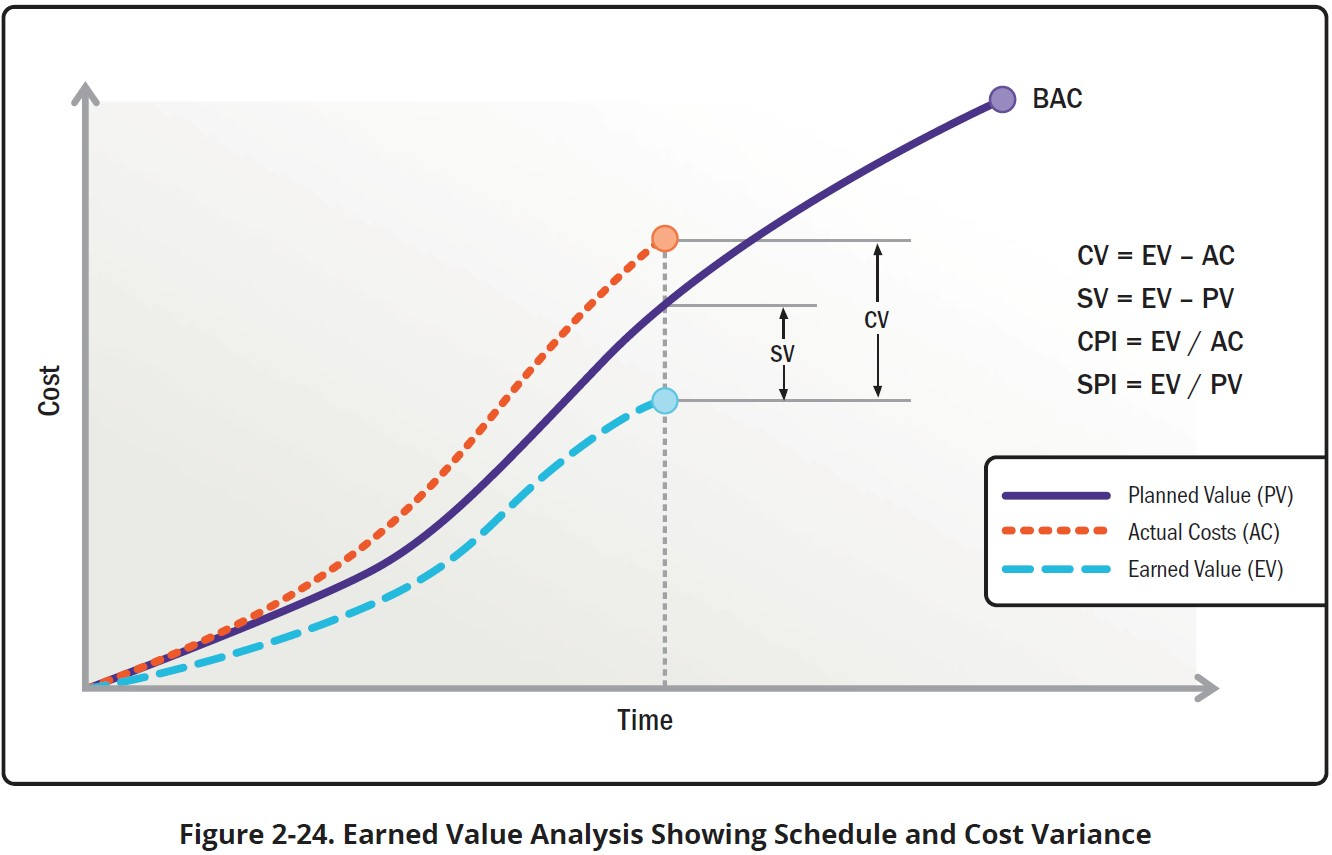
\includegraphics[width = 8cm]{../images/guide/Fig2-24.jpg}
    \label{guidefig:2-24}
 \end{figure}
\end{frame}
\begin{center}\line(1,0){250}\end{center}

\begin{frame}
\frametitle{Project ????}
 \begin{figure}
    \centering
        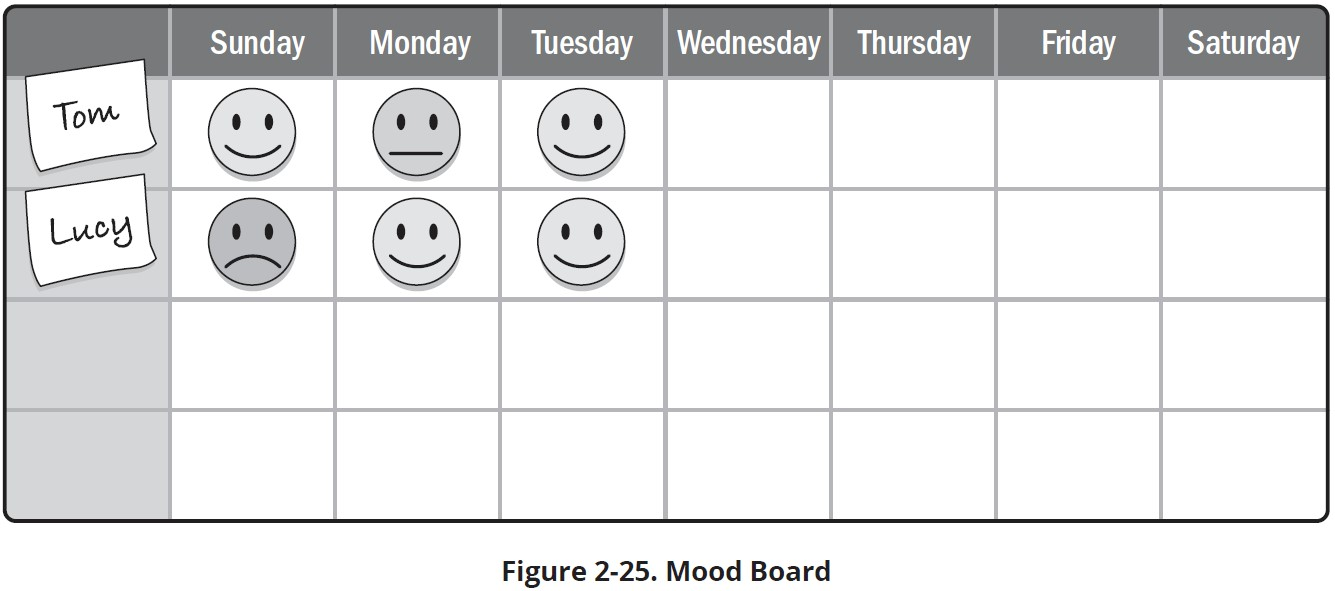
\includegraphics[width = 8cm]{../images/guide/Fig2-25.jpg}
    \label{guidefig:2-25}
 \end{figure}
\end{frame}
\begin{center}\line(1,0){250}\end{center}

\begin{frame}
\frametitle{Project ????}
 \begin{figure}
    \centering
        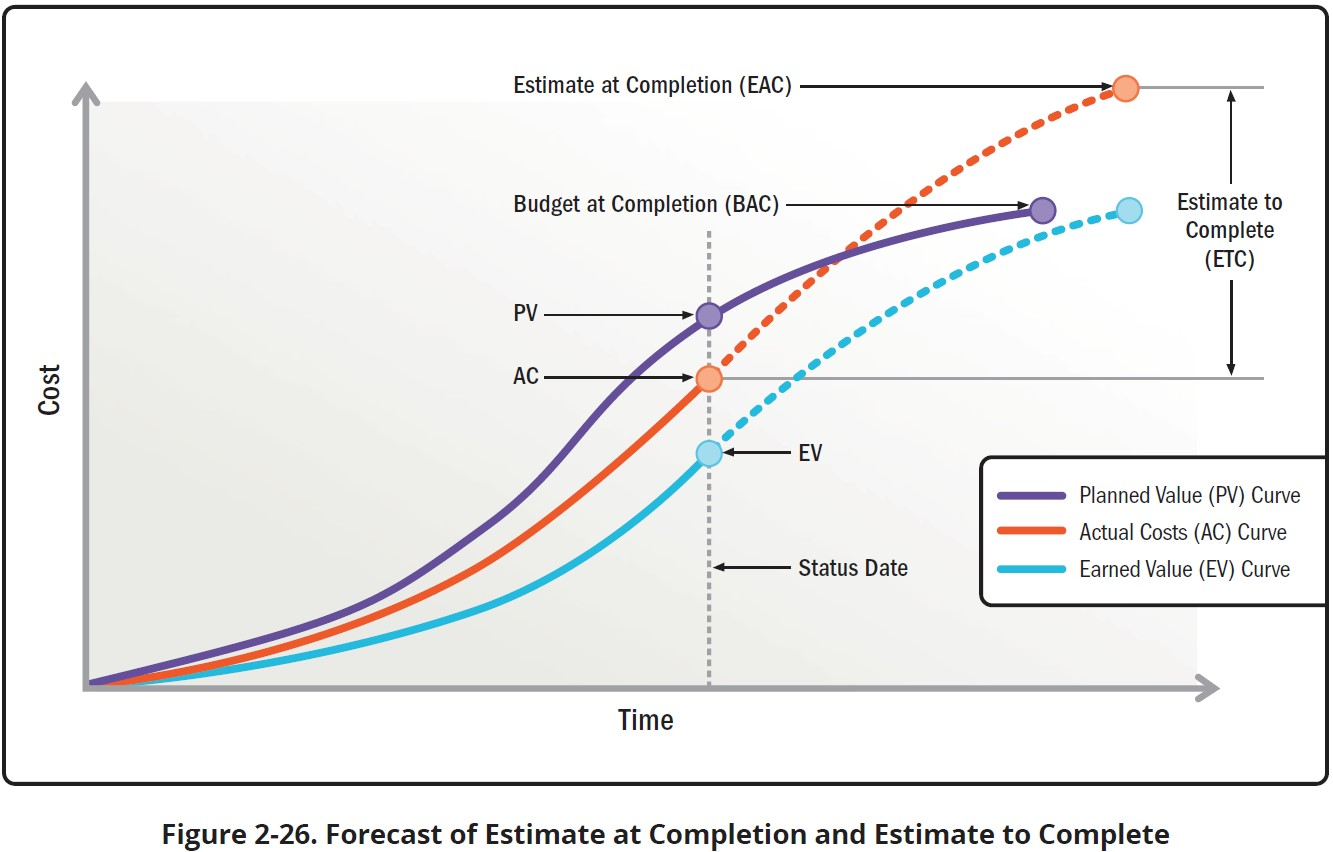
\includegraphics[width = 8cm]{../images/guide/Fig2-26.jpg}
    \label{guidefig:2-26}
 \end{figure}
\end{frame}
\begin{center}\line(1,0){250}\end{center}

\begin{frame}
\frametitle{Project ????}
 \begin{figure}
    \centering
        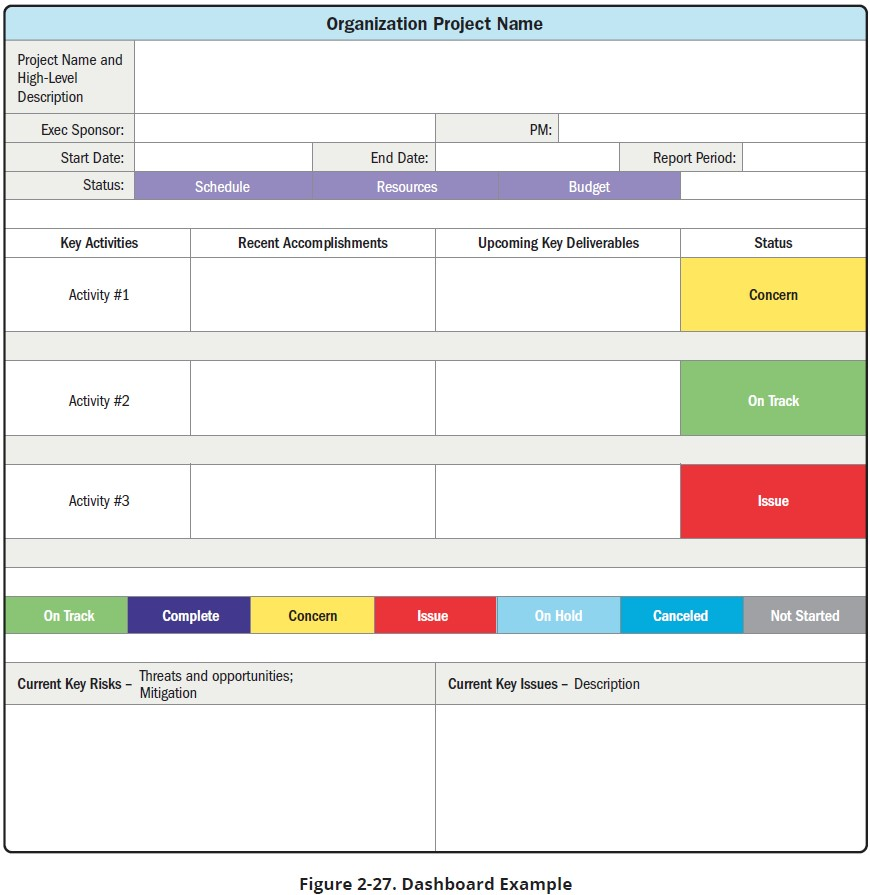
\includegraphics[width = 6cm]{../images/guide/Fig2-27.jpg}
    \label{guidefig:2-27}
 \end{figure}
\end{frame}
\begin{center}\line(1,0){250}\end{center}

\begin{frame}
\frametitle{Project ????}
 \begin{figure}
    \centering
        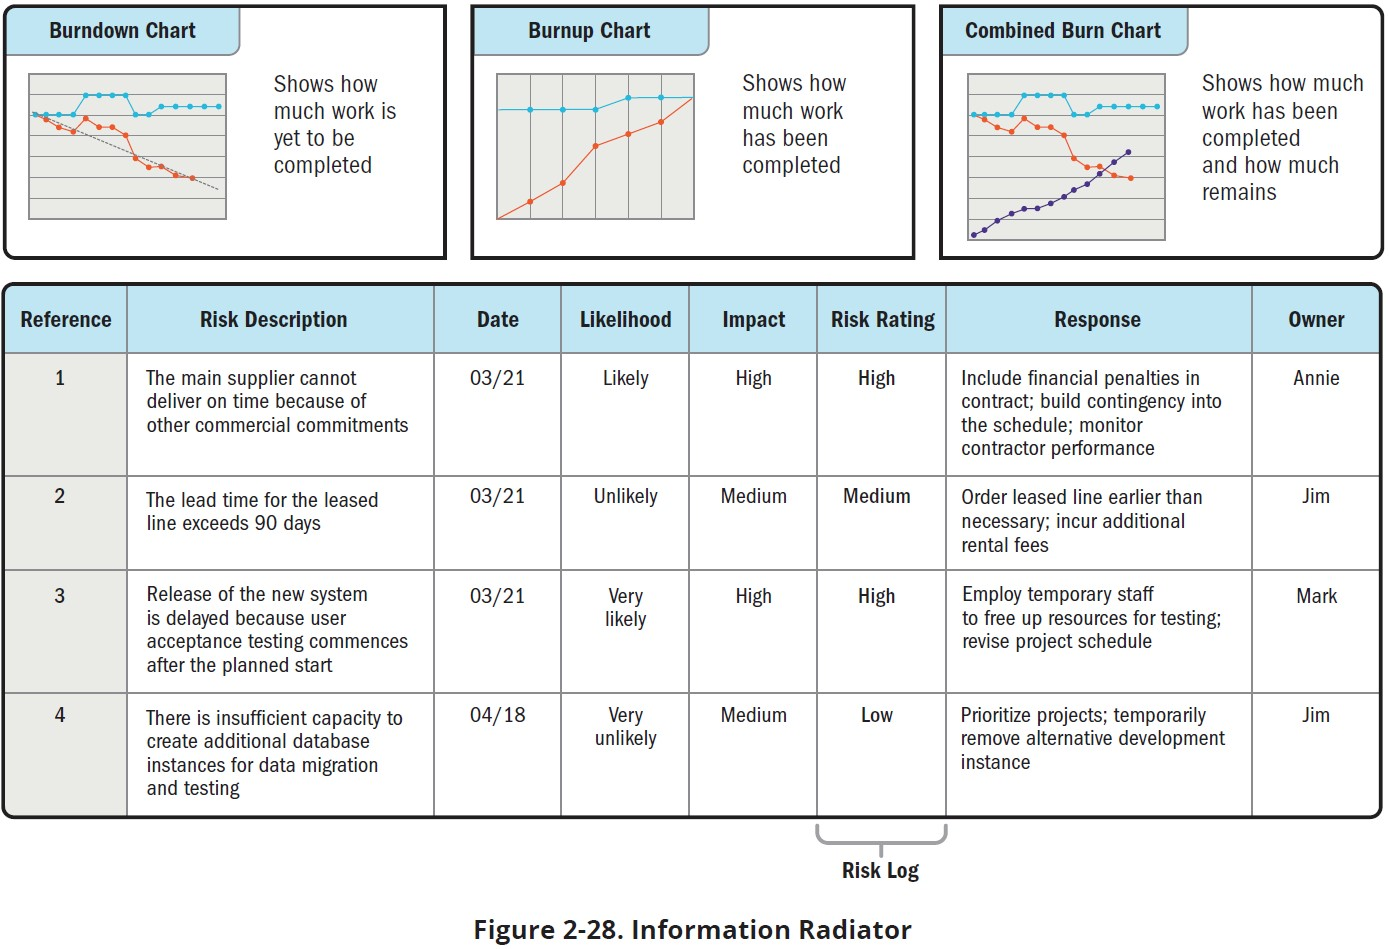
\includegraphics[width = 8cm]{../images/guide/Fig2-28.jpg}
    \label{guidefig:2-28}
 \end{figure}
\end{frame}
\begin{center}\line(1,0){250}\end{center}

\begin{frame}
\frametitle{Project ????}
 \begin{figure}
    \centering
        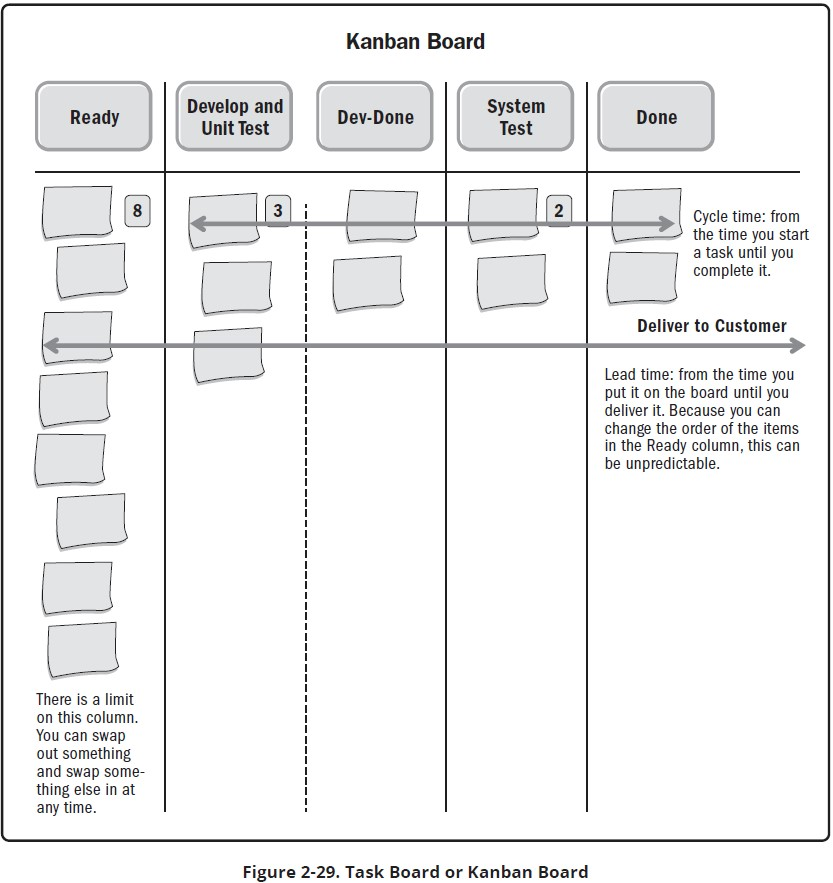
\includegraphics[width = 6cm]{../images/guide/Fig2-29.jpg}
    \label{guidefig:2-29}
 \end{figure}
\end{frame}
\begin{center}\line(1,0){250}\end{center}

\begin{frame}
\frametitle{Project ????}
 \begin{figure}
    \centering
        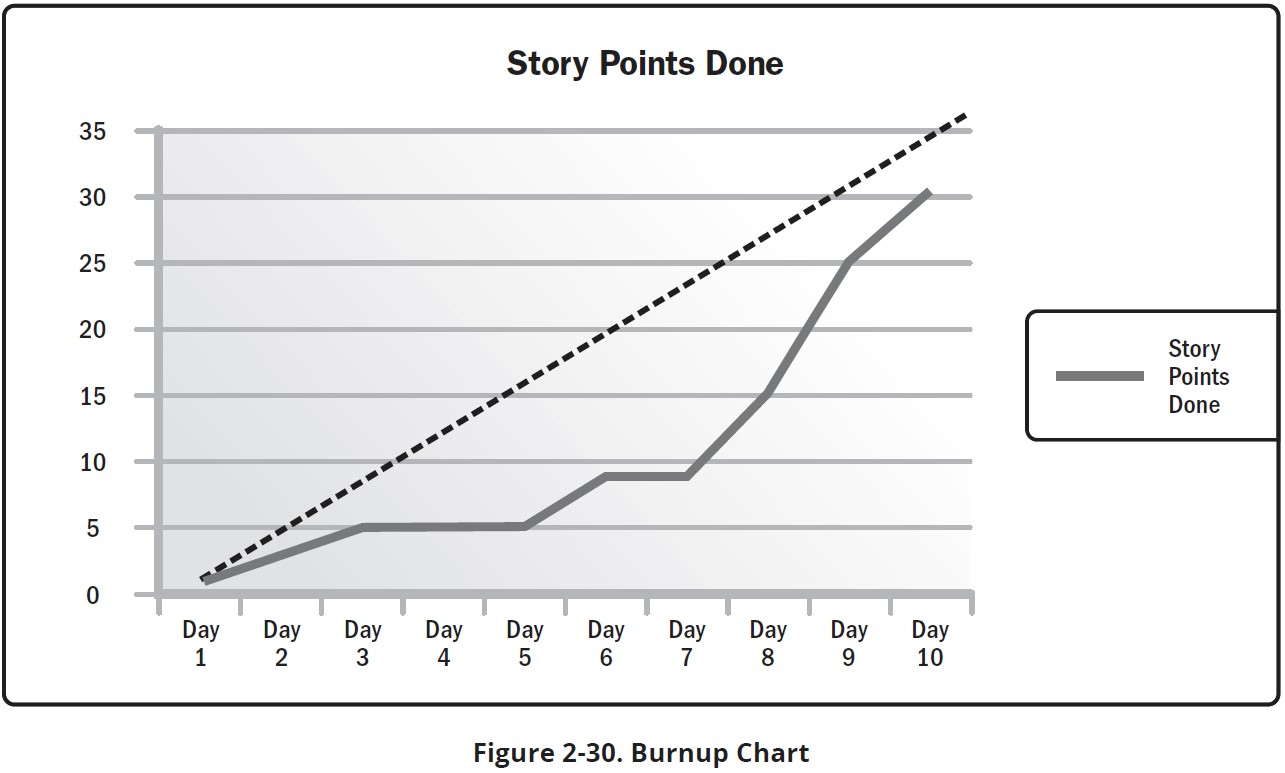
\includegraphics[width = 8cm]{../images/guide/Fig2-30.jpg}
    \label{guidefig:2-30}
 \end{figure}
\end{frame}
\begin{center}\line(1,0){250}\end{center}

\begin{frame}
\frametitle{Project ????}
 \begin{figure}
    \centering
        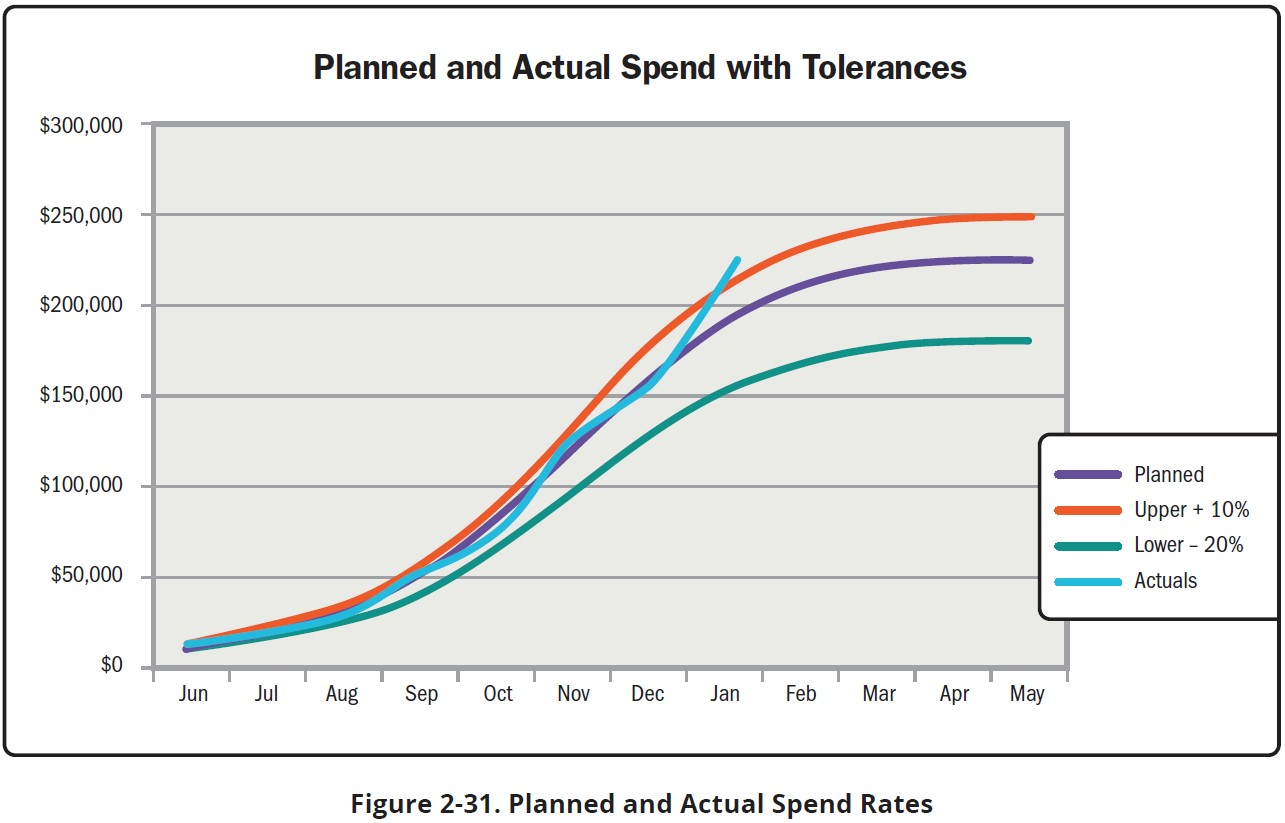
\includegraphics[width = 8cm]{../images/guide/Fig2-31.jpg}
    \label{guidefig:2-31}
 \end{figure}
\end{frame}
\begin{center}\line(1,0){250}\end{center}


\begin{frame}
\frametitle{Project ????}
 \begin{figure}
    \centering
        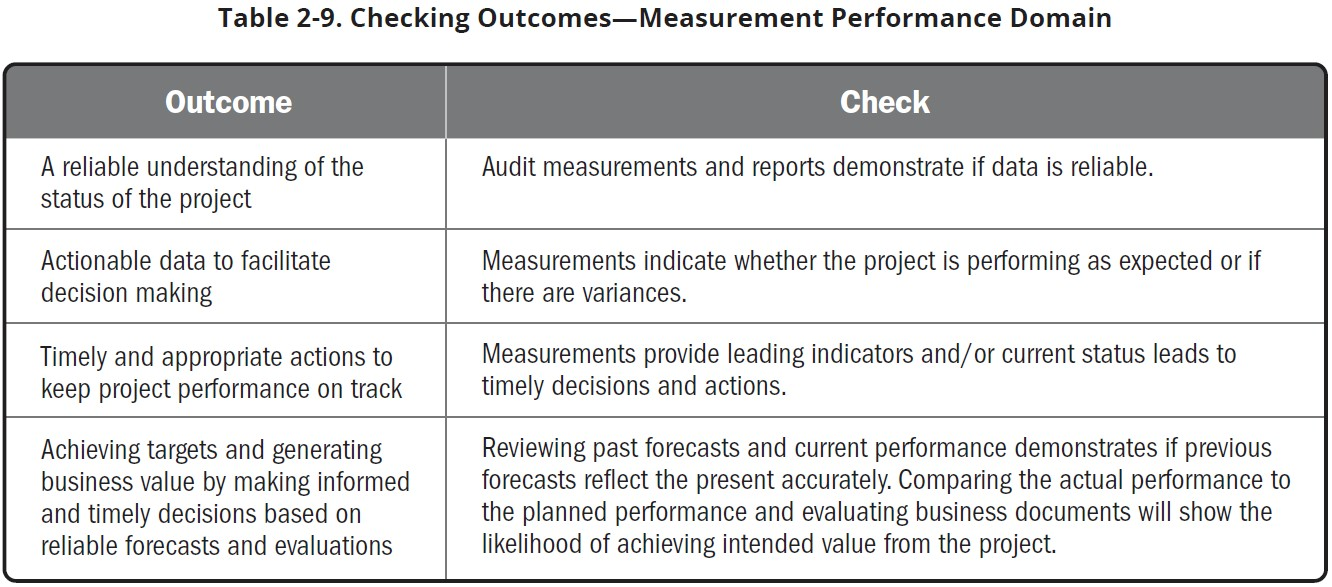
\includegraphics[width = 8cm]{../images/guide/Table2-9.jpg}
    \label{guideTable:2-9}
 \end{figure}
\end{frame}
\begin{center}\line(1,0){250}\end{center}



\end{document}
